\section*{Discussion}

While the points on Figure \ref{fig:procplot} are visibly correlated and have a strong correlation coefficient with the plotted regression, the shape of the points suggests the current induced in the wire and the force measured are closely but not linearly related.
Given that the random error is too small to result in meaningful differences, this means that either there exists systematic error in the experiment, or the hypothesis that current is linearly related to force is incorrect.

There are a few possibilities that could have led to the deviation from the hypothesis, of which one is friction.
Friction between the hooks of the wire and the hinges of the supports would create resistance torque which would set a force threshold before the wire can deflect.
however, the resistance torque should not increase as the deflection angle increases.
This is because, as the deflection angle increases, the weight of the wire will become distributed between the supports and the end of the vertical length of the wire (the bottom of the wire), of which will be supported by the Lorentz force.
In addition, friction was considered in the procedure, where the hinges had to be loose enough to allow the wire to swing freely.
Given an analysis of torque on the experiment is beyond the scope of this investigation, the best guess that can be given is that friction is insignificant to the results of the experiment.

Another possibility is the experiment failed to consider the force of attraction between the supports and the wire.
Since both are conductors and have current flowing between them, they will create a magnetic field that will influence the other, hence experience attraction or repulsion between each other.
Knowing from Lorentz force, if current in one wire is going the opposite direction of current in the other wire, they will repel each other, which could attribute to a slight increase in force at lower deflection angles.
The force exerted between the two wires can be estimated by using the definition of the ampere:
``One ampere is defined as the current that would cause a force of $2 \times 10^{-7}\si{\newton}$ per metre between two long parallel conductors separated by $1\si{\meter}$ in a vacuum.''\footcite{pearsonamp}
Right away, $2 \times 10^{-7}\si{\newton}$ is three orders of magnitude below the measured force, meaning that, even with one ampere going through the wire, the contributing force would be unnoticeable.
This means the attraction between the supports and the wire is not the main cause of the deviation from a linear relation in the experiment.

Since, the horizontal segment of the wire did vary in distance between the magnets, it is possible that the B-field varied by a significant amount as the wire swung during the experiment.
Although magnetic field strength does not exactly follow the inverse square law, its strength still decreases substantially with distance.
At the minimum and maximum deflection angles (around $5\si{\degree}$ or $30\si{\degree}$) the magnetic field could have been stronger than the rest of the angles.
However, the opposite is reflected in the data in Figure \ref{fig:procplot}, as force at the low and high currents are below the linear regression, while points in the middle are above the linear regression.
This does not mean variation in magnetic field strength is ruled out.
There is the possibility that, despite using large magnets, the magnetic field strength between the two magnets was not uniform; while the field lines were perpendicular to the surface of the magnets, the density of the field lines was concentrated near the center of the magnets.
Using the magnetic gap calculator from K{\&}J Magnetics, the magnetic field strength relative to the distance from the center axis between two cylindrical magnets can be determined.\footcite{kjgap}
By approximating the dimensions of the experiment magnets as cylindrical magnets and setting an arbitrary magnetic field strength (of similar composition to the magnets used in the experiment), the graph in Figure \ref{fig:gaps} was produced.
\begin{figure}[H]
	\centering
	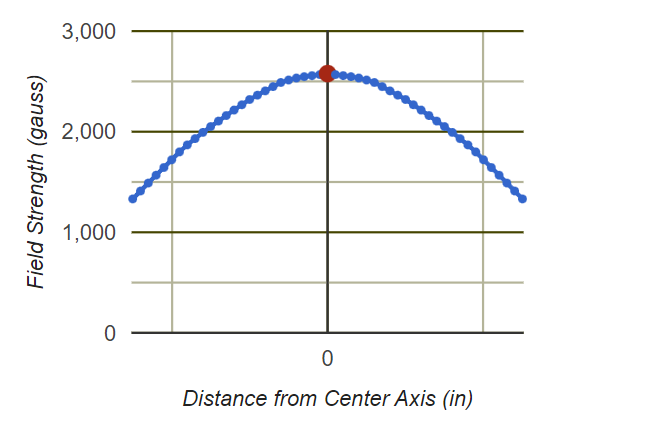
\includegraphics[width=0.5\textwidth]{figures/gapplot.PNG}
	\caption{Distribution of field strength over distance from the center axis between two magnets.}
	\label{fig:gaps}
	\vspace{-1em}
\end{figure}
This would explain why the force at the minimum and maximum angles varies from a linear relation; the magnetic field strength decreases when the wire is further away from the center.
While the geometry between rectangular and cylindrical magnets are different, it is likely this concept is still present in rectangular magnets.
Therefore, the variation of the data from a linear relation is due to the uneven distribution of the magnetic field between the two magnets.

\section*{Evaluation}

A major weakness to this experiment is the lack of magnetic field measurement.
Because the magnetic flux density was not evenly distributed throughout the magnetic field, thus leading to the non-linear relation, it is difficult to determine if the data supports the hypothesis.
While it is possible to correct the data based on the flux of the magnets used, all that is known is that they are ferrite magnets; their grades are unknown, hence their flux density cannot be determined.
Had a magnetic field probe been used to measure the magnetic field strength, it would have not only been possible to determine the field strength profile of the magnets, but also recognize the uneven distribution of field strength before the experiment took place.

The scale of the experiment had also posed some problems during the trials.
Of the negligible forces detailed in the discussion, the friction in the hinges caused issues with the measurements.
Fluctuations in current made it difficult to measure around the target values and sometimes required manual intervention to reduce the swinging.
This can be attributed to the use of a small lightweight wire, which was originally intended to reduce inertia.
While this means friction was be at a minimum, this also means there is more freedom to ``jiggle'' around, changing points of contact with the support and leading to inconsistent current.
This problem could be resolved by using copper tape and a copper rod.
The tape would allow for more flexibility and behave similar to string, permitting it to pivot freely and maintain a more constant contact with a hinge.
And a copper rod will ensure the center of mass is closer to the furthest end of the pendulum from the pivot, as well as increasing the weight to make sure the tape stays in contact with the hinge.

Additionally, as mentioned in the qualitative observations, the wire would get close to the bracket at high deflection angles.
The proximity of the wire to the bracket and the magnets means the magnetic field strength experienced by the wire was greater.
This is reflected in the data where high angle measurements are minutely skewed, as seen at $1.40\si{\ampere}$ on Figure \ref{fig:procplot}, where the data points seem to have a slightly higher rate of increase compared to other data points.
The issue of proximity can again be attributed to the compactness of the experiment design.
Due to limitations in the available magnets for this experiment, the wire had roughly $3.4\si{\centi\meter}$ of distance to swing freely, restricted by the dimensions of the magnets.
Either larger magnets or changing the placement of the bracket would remedy this issue.

The random error in this experiment was kept at a minimum through the use of precise equipment and minimizing the number of variables which needed to be multiplied together, reducing the scale factor of error as much as possible. 
While the largest source of random error was the mass of the wire, $\pm0.1\si{\gram}$, it is only a singular measurement, meaning that its true measurement affects every data point, thus not affecting the mathematical relationship.
Because the angle measurements were done using a camera, necessitated by the fact that a protractor would be difficult to hold to such a small setup, there is the possibility of the measurements being incorrect due to lens distortion.
However, this was considered during the procedure, and if the camera was facing down, perpendicular to the length of the horizontal segment of the wire, did not change position or orientation, and was kept at a constant distance, then lens distortion should not be a problem.
